\documentclass[USenglish,pdftex,compress,10pt,svgnamesi,handout]{beamer}
%\documentclass[USenglish,pdftex,compress,10pt,svgnames]{beamer}
%\documentclass[notes,10pt,svgnames]{beamer}
\usepackage{import}\subimport{../../common/}{lectureheader}

\graphicspath{{pics/}}
\usepackage{listings}

\parskip2ex
\usepackage{tabu}

\newcommand{\bfw}{\Vec{w}}
\newcommand{\bfx}{\Vec{x}}
\newcommand{\bfz}{\Vec{z}}
\newcommand{\bfg}{\Vec{g}}
\newcommand{\bfu}{\Vec{u}}
\def\bf#1{\Vec{#1}}
\def\cl#1{{\cal #1}}
\DeclareMathOperator{\sgn}{sgn}
\def\hid{{H}}


% =====================================================================
% Titel etc.
\hypersetup{%
	pdftitle={neural networks: advanced models},%
	pdfauthor={Patrick van der Smagt}%
}

\title{neural networks: advanced models}
\author{Patrick van der Smagt}
\date{}
% =====================================================================
\begin{document}


%'''''''''''''''''''''''''''''''''''''''''''''''''''''''''
\begin{frame}
	\titlepage
	
	\vfil
\end{frame}



\begin{frame}
\frametitle{image processing with neural networks}

Since 2009, convolutional neural networks (cNN aka ConvNet) have  beaten many computer vision benchmarks.
cNNs were somehow modelled after an abstract model of the human visual cortex, but have since progressed away from that.

A typical cNN consists of stacked convolutional and maxpooling layers.
\begin{columns}
\begin{column}{0.7\textwidth}
\begin{itemize}
\item a convolutional layer consists of a number of $n\times m$ filters which are convolved on the image. For instance, a $5\times5$ filter is matched on all positions of the image, and the result of this match is the next image.  This is done for many different filters (see figure);
\item a maxpooling layer downsamples the resulting images, typically in $2\times2$ windows.
\end{itemize}
This structure is stacked, typically 2 to 4 times.
\end{column}
\begin{column}{0.25\textwidth}
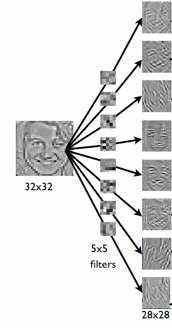
\includegraphics[width=\textwidth]{convol}
\end{column}
\end{columns}
The power of a cNN is that the convolution filters are \textsl{learned}.

\end{frame}



\begin{frame}
\frametitle{convolutional deep learning example (Ng 2009)}
\begin{center}
first layer (top) and second layer (bottom) weights for selected images 
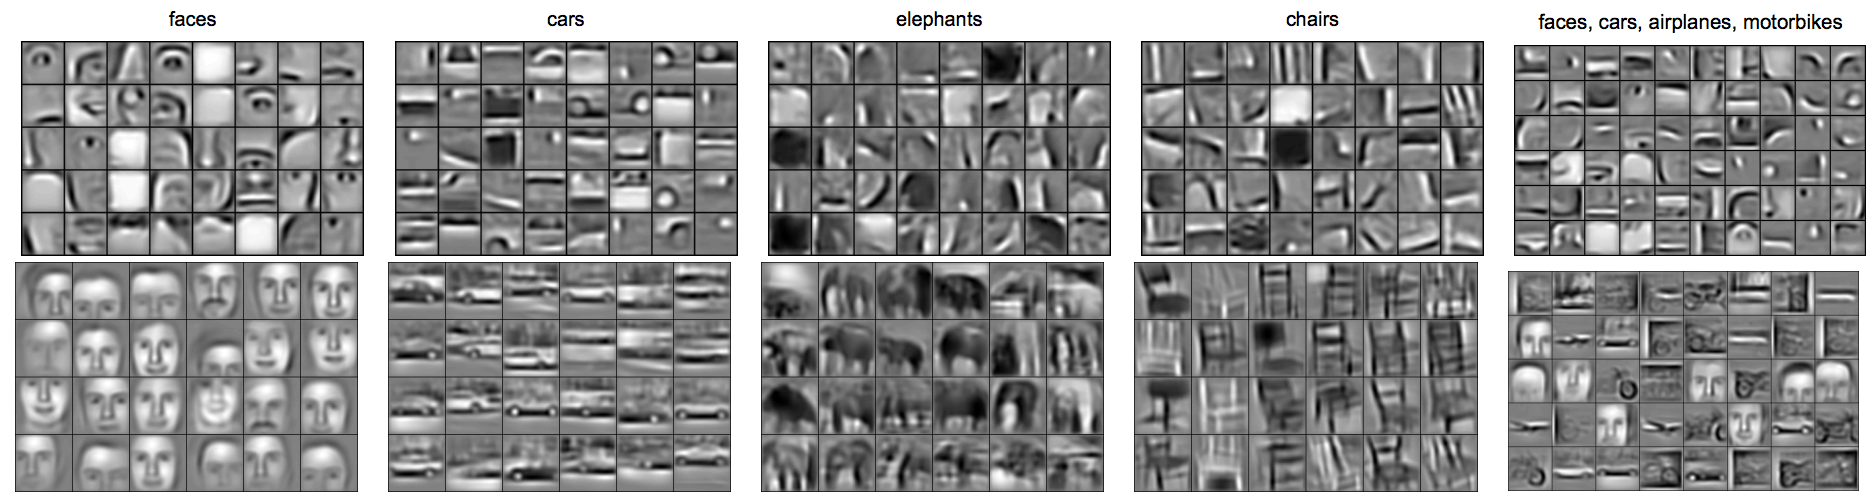
\includegraphics[width=0.99\textwidth]{pics/ng2009-1.png}

 for natural images \\
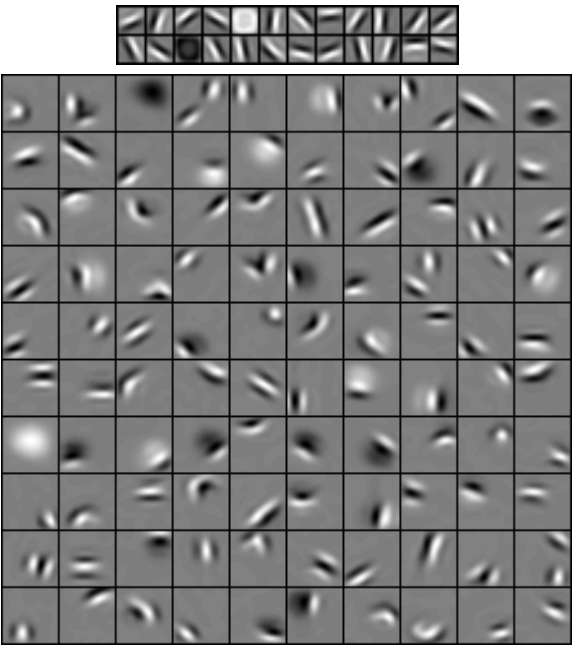
\includegraphics[height=4cm]{pics/ng2009-2.png}
\end{center}
\end{frame}



%
%
%\begin{frame}
%\frametitle{variational inference}
%
%Let us assume we want to model $p(\Vec z \mid \Vec x)$.
%
%We choose a prior $p(\Vec z)$: that is the distribution that we want our data to adhere to.
%
%We can only find $p(\Vec z \mid \Vec x)$ through sampling, which is too expensive.
%
%So we approximate $p(\Vec z \mid \Vec x)$ by $q(\Vec z \mid \Vec x, \Vec w)$. 
%
%To make the distributions similar, we minimise the KL divergence
%$
%\KL{q(\Vec z \mid \Vec x, \Vec w)}{p(\Vec z \mid \Vec x)}
%$
%which we can simplify to 
%$$
%\KL{q(\Vec z \mid \Vec x, \Vec w)}{p(\Vec z \mid \Vec x)}
%=
%\log p(\Vec x)  + \mathcal{L}(\Vec w)
%$$
%where $ \mathcal{L}(\Vec w)$ is the loss (cq.\ the negative log-likelihood). 
%
%\end{frame}
%
%
%
%
%\begin{frame}
%\frametitle{variational inference}
%We thus find that
%$$\log p(\Vec x) = \KL{q(\Vec z \mid \Vec x)}{p(\Vec z \mid \Vec x)} -  \mathcal{L}(\Vec w) $$
%
%
%\end{frame}
%
%
%
%
%\begin{frame}
%\frametitle{probabilistic neural networks}
%\end{frame}
%
%
%
%
%\begin{frame}
%\frametitle{probabilistic neural networks}
%\end{frame}
%
%
%
%
%\begin{frame}
%\frametitle{probabilistic neural networks}
%\end{frame}
%
%




\frame{\frametitle{unsupervised learning with neural networks}
\ParBeg{problem:} often we have unlabelled data
\begin{enumerate}
	\item we have many data $\Vec x$\dots
	\item but no related output $\Vec z$.
\end{enumerate}
\medskip

\begin{columns}
\column{0.3\textwidth}
%\imgbox{VAE-half}{}{\textwidth}
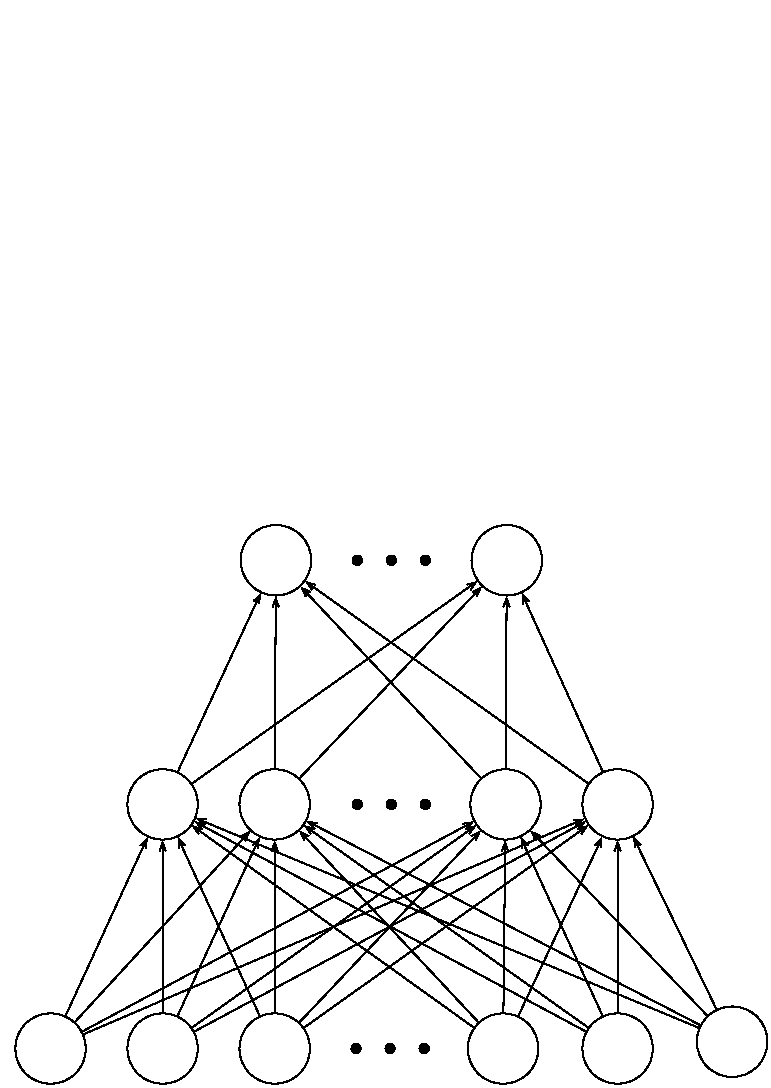
\includegraphics[width=\textwidth]{VAE-half}
\column{0.7\textwidth}
\end{columns}
\vfill
}




\frame{\frametitle{auto-encoder networks}
\ParBeg{idea:} find compact representation of inputs (unsupervised!)\ by
\begin{enumerate}
	\item stacking a second neural network on top of the first
	\item letting the whole NN compute $\Vec y(\Vec x) = \Vec x$.
\end{enumerate}
\medskip

\begin{columns}
\column{0.3\textwidth}
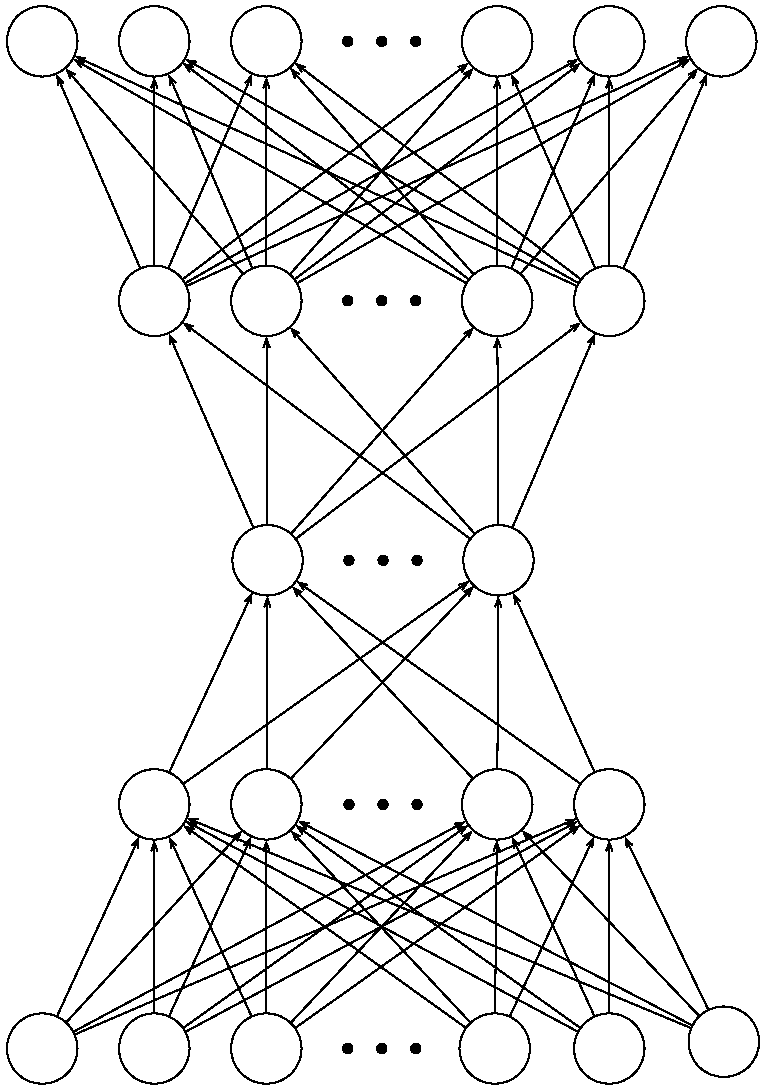
\includegraphics[width=\textwidth]{VAE}
\column{0.7\textwidth}
\begin{itemize}
  \item middle layer (``latents'') usually has fewer neurons 
  \item latent representation $\Vec z$ = compact code for $\Vec{x}$
\end{itemize}
\end{columns}
These networks make a compact representation of data (``dimensionality reduction'').
However, you cannot control the representation!

}


\begin{frame}
\frametitle{recurrent neural networks}

\begin{columns}
\column{0.25\textwidth}
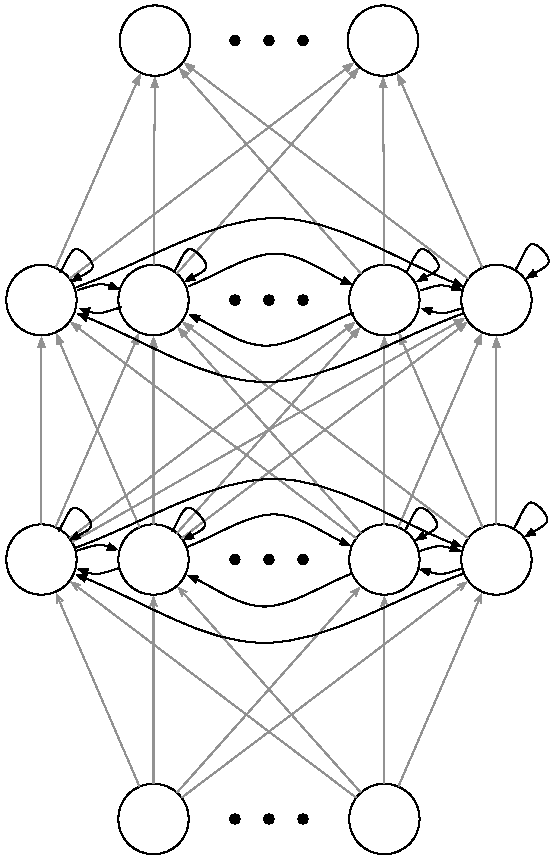
\includegraphics[width=0.8\textwidth]{RNN}

\centerline{RNN}
\column{0.2\textwidth}\centerline{=}
\column{0.45\textwidth}
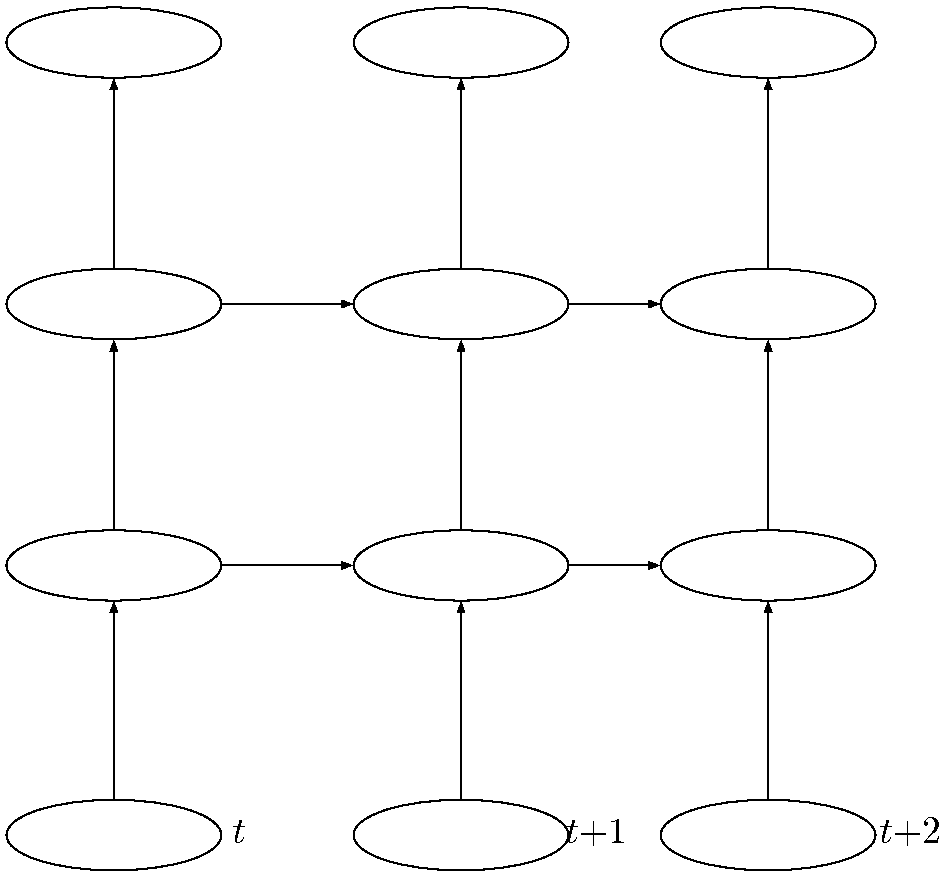
\includegraphics[width=0.8\textwidth]{RNN-rollout}

\centerline{rolled out in time}
\end{columns}
\vskip5mm
Can be trained with backpropagation-through-time:
\begin{itemize}
\item input a finite sequence  $\{\Vec x(t)\}$, $t = 1, 2, \dots T$ step by step
\item back-propagate the error $y(\Vec x(t)) - \Vec z(t)$ timestep by timestep, starting at $T$ down to 1, and sum the residuals;
\item adapt the weights using the residuals computed above.
\end{itemize}
\end{frame}



\begin{frame}
\frametitle{recurrent neural networks}
RNNs have been successfully used for a number of serious applications.  

These include 
\begin{itemize}
 \item robotics;
 \item handwritten character recognition and generation;
 \item text recognition, generation, annotation, etc.; speech recognition;
 \item machine translation
\end{itemize}
and so on.

\end{frame}








\begin{frame}
\frametitle{probabilistic neural networks}

Neural networks become much more powerful if they are probabilistic.
In these, each neuron represents a random variable rather than a value.
In cleartext, a neuron in fact represents a mean and a variance, i.e., two values rather than one are learned.

The probabilistic neural network introduce many possibilities:
\begin{itemize}
  \item prediction of confidence intervals at the output;
  \item probabilistic version of dropout;
  \item towards a full probabilistic interpretation;
  \item \dots
\end{itemize}

\end{frame}


%\begin{frame}
%\frametitle{probabilistic neural networks}
%
%%$$
%%p(\Vec\target\mid\Vec x) = \int_{\Vec w}  p(\Vec\target\mid\Vec x, \Vec w) \, p(\Vec w \mid D_t)\, d \Vec w
%%$$
%Let  the summed input of a neuron be $a=\Vec w^T \Vec x$, and its output $y=\phi(a)$. 
%The activation of the neuron is given by
%$$
%p(a\mid\Vec x) =
% \int_{\Vec w} q(\Vec w) \, p(a \mid \Vec x, \Vec w) \, d\Vec w
%$$
%where $q$ is some distribution over the parameters $\Vec w$.
%
%Assuming that $\Vec w$, $\Vec x$ are independent and ``large enough'', the central limit theorem applies and $q$ is a Gaussian.  So
%$$
%p(a\mid\Vec x) =
% \int_{\Vec w} q(\Vec w) \, p(a \mid \Vec x, \Vec w) \, d\Vec w
% \approx \N(\E(a), \var(a))
%$$
%with
%\begin{align}
%\E(a) &= \E(\Vec w)^T \E(\Vec x),\\
%\var(A) &= \sum_i \var(w_i x_i) = \dots \\&= \var(\Vec w)^T\E(\Vec x)^2 + \var(\Vec x)^T \E(\Vec w)^2 + \var(\Vec x)^T \var(\Vec w)
%\end{align}
%\end{frame}
%
%
%
%
%\begin{frame}
%\frametitle{probabilistic neural networks}
%So if $a$ is Gaussian, what is $y=\phi(a)$?
%Well, for instance for a sigmoid activation function,  it can be derived that 
%\begin{align}
%\E(y) &\approx \sigma(\E(a), \var(a))\\
%\var(y) &\approx\sigma(a\E(a), a^2\var(a)) - \E(a)^2
%\end{align}
%
%This can be generalised to all neurons in a neural network.
%
%\vfill
%
%These equations allow for learning $\E(x), \var(x)$ given a prior distribution, and a probabilistic representation of the neural network is possible.
%\end{frame}
%

%
%\begin{frame}
%\frametitle{Deep autoencoder Example: Face Compression}
%\begin{center}
%\includegraphics[width=0.9\textwidth]{pics/hinton1.png}
%\end{center}
%\end{frame}
%%%
%\begin{frame}
%\frametitle{Deep autoencoder Example: Text Categorisation}
%\begin{center}
%\includegraphics[width=0.99\textwidth]{pics/hinton2.jpg}
%\end{center}
%\end{frame}









%\frame{\frametitle{the transfer function}
%  \begin{columns}
%    \begin{column}{5.0cm}
%The response of a simulated neuron to its activation $a_j$ is given by a \alert{transfer function}
%$$
%o_j = \phi_j(a_j)
%$$
%\vfill
%    \end{column}
%    \begin{column}{4.0cm}
%			\hfill\imgbox{trafctneuron}{}{4.0cm}
%		\end{column}
%  \end{columns}
%
%In the simplest case, the transfer function can be selected to be the identity function, or another linear function. However, in order for the network to exhibit nonlinear properties, $\phi(\cdot)$ also has to be nonlinear.
%}
%
%\frame{\frametitle{the transfer function}
%\begin{itemize}
%	\item historically, binary and piecewise linear transfer functions were
%		chosen first, in reference to the threshold-like behaviour of biological neurons
%	\pause
%	\item smooth, S-shaped (=\alert{sigmoid}) functions behave like
%		threshold or linear functions, depending on scaling, and can be differentiated
%	\pause
%	\item another network class, radial basis function (RBF) networks,
%		uses Gaussian-shaped transfer functions.
%\end{itemize}
%
%}
%
%\frame{\frametitle{commonly used transfer functions}
%\imgbox{transferfct}{}{\textwidth}
%}
%

%%%%
%\begin{frame}[fragile]
%\frametitle{better algorithm for backprop (``(mini) batch learning'')}
%
%\begin{beamerboxesrounded}[upper=def,lower=block body,width=1.03\textwidth,shadow]{\textbf{back-propagation algorithm:}}
%\begin{lstlisting}[mathescape]
%initialise the weights
%repeat
%  randomly select samples $(\bfx,\bfz)$ from a mini-batch do
%  begin
%     $\bf o = \cl M(\bfw, \bfx)$; forward pass
%     calculate error $\bfz  - \bf o$ at the output units
%     for all $w^{(2)}$ compute $\delta_{w^{(2)}}$; backward pass
%     for all $w^{(1)}$ compute $\delta_{w^{(1)}}$; backward pass continued
%     sum the delta weights using $\partial E / \partial w_{ij} = \delta_{j} x_{i}$
%  end
%  update the weights using summed delta weights
%until stopping criterion satisfied
%\end{lstlisting}
%\end{beamerboxesrounded}
%\end{frame}

%%%%%%%%%%%%%%




%\begin{frame}
%\frametitle{Minkowski-R error }
%We previously assumed Gaussian distribution of the target values by
%$$
%p(\epsilon) = { 1 \over \sqrt{2\pi\sigma^2}} \exp\left(-{\epsilon^2\over 2 \sigma^2}\right)
%$$
%\pause
%If we take the more general form
%$$
%p(\epsilon) = { R \beta^{1/R} \over 2 \Gamma (1/R)} \exp\left(-\beta |\epsilon|^R\right)
%$$
%The likelihood of the prior leads to minimisation of 
%$$
% E(\bfw) = {1 \over 2} \sum _{p=1}^{n} \left|\bfz_{p} - \cl M(\bfw, \bfx_{p})\right|^R
% $$
%\end{frame}






\begin{frame}{What is a transformer?}
\begin{itemize}
    \item A transformer is a neural network architecture that was proposed by Vaswani et al. (2017) for natural language processing tasks.
    \item It is based on the idea of self-attention, which is a mechanism that allows the network to learn the relationships between different parts of the input sequence.
    \item A transformer consists of two main components: an encoder and a decoder. The encoder processes the input sequence and generates a representation for each token. The decoder generates the output sequence by attending to the encoder representation and its own previous outputs.
    \item A transformer can handle variable-length inputs and outputs without using recurrent or convolutional layers, which makes it more efficient and scalable.
\end{itemize}
\end{frame}

\begin{frame}{How does a transformer work?}
\begin{figure}
    \centering
    \begin{tikzpicture}[node distance=1cm]
        \node (input) [draw, rectangle] {Input};
        \node (encoder) [draw, rectangle, right=of input] {Encoder};
        \node (decoder) [draw, rectangle, right=of encoder] {Decoder};
        \node (output) [draw, rectangle, right=of decoder] {Output};
        \draw [->] (input) -- (encoder);
        \draw [->] (encoder) -- (decoder);
        \draw [->] (decoder) -- (output);
        \draw [->] (decoder) to [out=135,in=45,looseness=2] node[above] {Self-attention} (decoder);
        \draw [->] (decoder) to [out=225,in=315] node[below] {Cross-attention} (encoder);
    \end{tikzpicture}
\end{figure}
\begin{itemize}
    \item The encoder and the decoder are composed of multiple layers, each containing a multi-head self-attention sublayer and a feed-forward sublayer with residual connections and layer normalisation.
    \item The self-attention sublayer allows each token to attend to all other tokens in the same sequence, and computes a weighted sum of their representations. The multi-head mechanism allows the network to learn different aspects of attention from different subspaces of the representation.
    \item The cross-attention sublayer allows each token in the decoder to attend to all tokens in the encoder, and computes a weighted sum of their representations. This enables the decoder to generate outputs that are relevant to the input.
    \item The feed-forward sublayer consists of two linear transformations with a non-linear activation function in between. It uses the same function to each token independently, and enhances the representation capacity of the network.
\end{itemize}
\end{frame}



\begin{frame}
\frametitle{transformers graphical model}

\resizebox{5cm}{!}{ \begin{tikzpicture}

% encoder nodes
\node[obs] (x1) {$x_1$};
\node[obs, right=of x1] (x2) {$x_2$};
\node[obs, right=of x2] (x3) {$x_3$};
\node[latent, above=of x1] (h1) {$h_1$};
\node[latent, above=of x2] (h2) {$h_2$};
\node[latent, above=of x3] (h3) {$h_3$};

% decoder nodes
\node[latent, right=of h3] (s1) {$s_1$};
\node[latent, right=of s1] (s2) {$s_2$};
\node[latent, right=of s2] (s3) {$s_3$};
\node[obs, below=of s1] (y1) {$y_1$};
\node[obs, below=of s2] (y2) {$y_2$};
\node[obs, below=of s3] (y3) {$y_3$};

% encoder edges
\edge {x1} {h1};
\edge {x2} {h2};
\edge {x3} {h3};
\edge {h1} {h2,h3,s1,s2,s3};
\edge {h2} {h1,h3,s1,s2,s3};
\edge {h3} {h1,h2,s1,s2,s3};

% decoder edges
\edge {s1} {y1,s2};
\edge {s2} {y2,s3};
\edge {s3} {y3};

% plates
\plate [inner sep=0.25cm,xshift=-0.12cm,yshift=0.12cm] {plate_x} {(x1)(x2)(x3)} {$N_x$};
\plate [inner sep=0.25cm,xshift=-0.12cm,yshift=0.12cm] {plate_y} {(y1)(y2)(y3)} {$N_y$};

\end{tikzpicture}}
\footnotesize

The nodes represent random variables and the edges represent conditional dependencies. The shaded nodes are observed variables and the unshaded nodes are latent variables. The plates indicate repeated variables.

In this graphical model, the input sequence is denoted by $x_1, x_2, \dots, x_{N_x}$ and the output sequence is denoted by $y_1, y_2, \dots, y_{N_y}$. The encoder generates a representation for each input token, denoted by $h_1, h_2, \dots, h_{N_x}$. The decoder generates a hidden state for each output token, denoted by $s_1, s_2, \dots, s_{N_y}$.

The edges from the input tokens to the encoder representations indicate that each $h_i$ depends on $x_i$. The edges from the encoder representations to the decoder hidden states indicate that each $s_j$ depends on all $h_i$'s. The edges from the decoder hidden states to the output tokens indicate that each $y_j$ depends on $s_j$. The edges from the decoder hidden states to the next decoder hidden states indicate that each $s_j$ also depends on the previous $s_{j-1}$.

The graphical model captures the conditional distribution of the output sequence given the input sequence:
$$p(y_1, y_2, \dots, y_{N_y} | x_1, x_2, \dots, x_{N_x})$$
\end{frame}


\begin{frame}
\frametitle{getting started}

Programming your own NN in Python is quite simple, but not efficient. 

For efficient code, use one of many public domain libraries, nowadays evolving around PyTorch, Tensorflow, JAX.  Which one will you choose?


Zillions of tutorials to be found.  For instance, check this recurrent neural network to translate between languages. \url{https://pytorch.org/tutorials/intermediate/seq2seq_translation_tutorial.html}

\end{frame}




%
%\begin{frame}
%\frametitle{Very recent developments}
%Deep Learning via Hessian-Free optimisation (J. Martens, ICML 2010)---add a regularisation
%term to the Hessian, i.e., $B=H+\lambda I$
%
%%Krylov Subspace Descent for Deep Learning (O. Vinyals and D. Povey, AISTATS 2012)
%
%Deep learning also works by training ordinary backprop ``ad infinitum'' 
%on \textsl{many} data (Cire\c san et al, 2010)---extend mnist by adding
%linearly convoluted versions of the images
%\end{frame}


\end{document}
